\subsection{Caméra embarquée}
\label{subsec:camera_logiciel}

Le logiciel embarqué a pour seule fonction de déclencher l'enregistrement des caméras après la mise sous tension de la carte.
La vidéo est ensuite stockée directement par les caméras et n'est pas traitée par l'ESP32 Xiao C3.

\subsubsection{Séquence de démarrage}

À la mise sous tension, le programme initialise l'ESP32 Xiao C3 et ses interfaces, puis démarre un compteur de \SI{10}{\minute}.
À l'issue de ce délai, les ordres de démarrage sont envoyés aux caméras. La séquence est donc la suivante :

\begin{enumerate}
    \item initialisation de la carte ;
    \item démarrage du compteur ;
    \item expiration du délai de \SI{10}{\minute} ;
    \item envoi des ordres de démarrage ;
    \item début de l'enregistrement.
\end{enumerate}

Après l'expiration du délai, le programme commande la RunCam Nano 2 par un changement d'état de son entrée High/Low. Il envoie
simultanément une commande de démarrage par UART aux RunCam Thumb Pro. Le même ordre est reçu par les deux Thumb Pro lorsqu'elles
partagent la ligne de réception.

\subsubsection{Développement du code}

Le protocole de commande UART a été repris à partir du dépôt RunCam Thumb ESP32-C3 Controller\cite{RunCam}, puis adapté au
fonctionnement de la carte. La temporisation de démarrage est fixée à \SI{10}{\minute}.\\

Les caméras enregistrent les vidéos sur leurs cartes SD et conservent les fichiers même lorsque leur alimentation est coupée.
Il n'est donc pas nécessaire de prévoir une commande d'arrêt spécifique en fin de vol. Lorsque les batteries arrivent en fin de
décharge, leur BMS coupe l'alimentation afin de les protéger. La carte caméra n'est alors plus alimentée et cesse à son tour
d'alimenter les caméras, sans que les vidéos déjà enregistrées soient perdues. La capacité des cartes SD permet de stocker
plusieurs heures de vidéo, soit une durée supérieure à l'autonomie des batteries. De plus, les caméras découpent les
enregistrements en fichiers de \SI{10}{\minute}, ce qui limite les risques de perte d'un enregistrement complet lors de la
coupure d'alimentation.\\

Des essais au sol ont permis de valider les ordres de déclenchement et d'arrêt, ainsi que la récupération des vidéos enregistrées.
La réception des commandes par les entrées de la PCB, après mise en forme par les triggers de Schmitt, a également été vérifiée.
Ces essais ont confirmé le fonctionnement de la chaîne de commande et de l'enregistrement vidéo.\\

La commande par les entrées n'a toutefois pas été utilisée pendant le vol. La configuration retenue reposait uniquement sur le
compteur de \SI{10}{\minute} intégré au logiciel de la carte caméra.

\newpage

\begin{figure}[H]
    \centering
    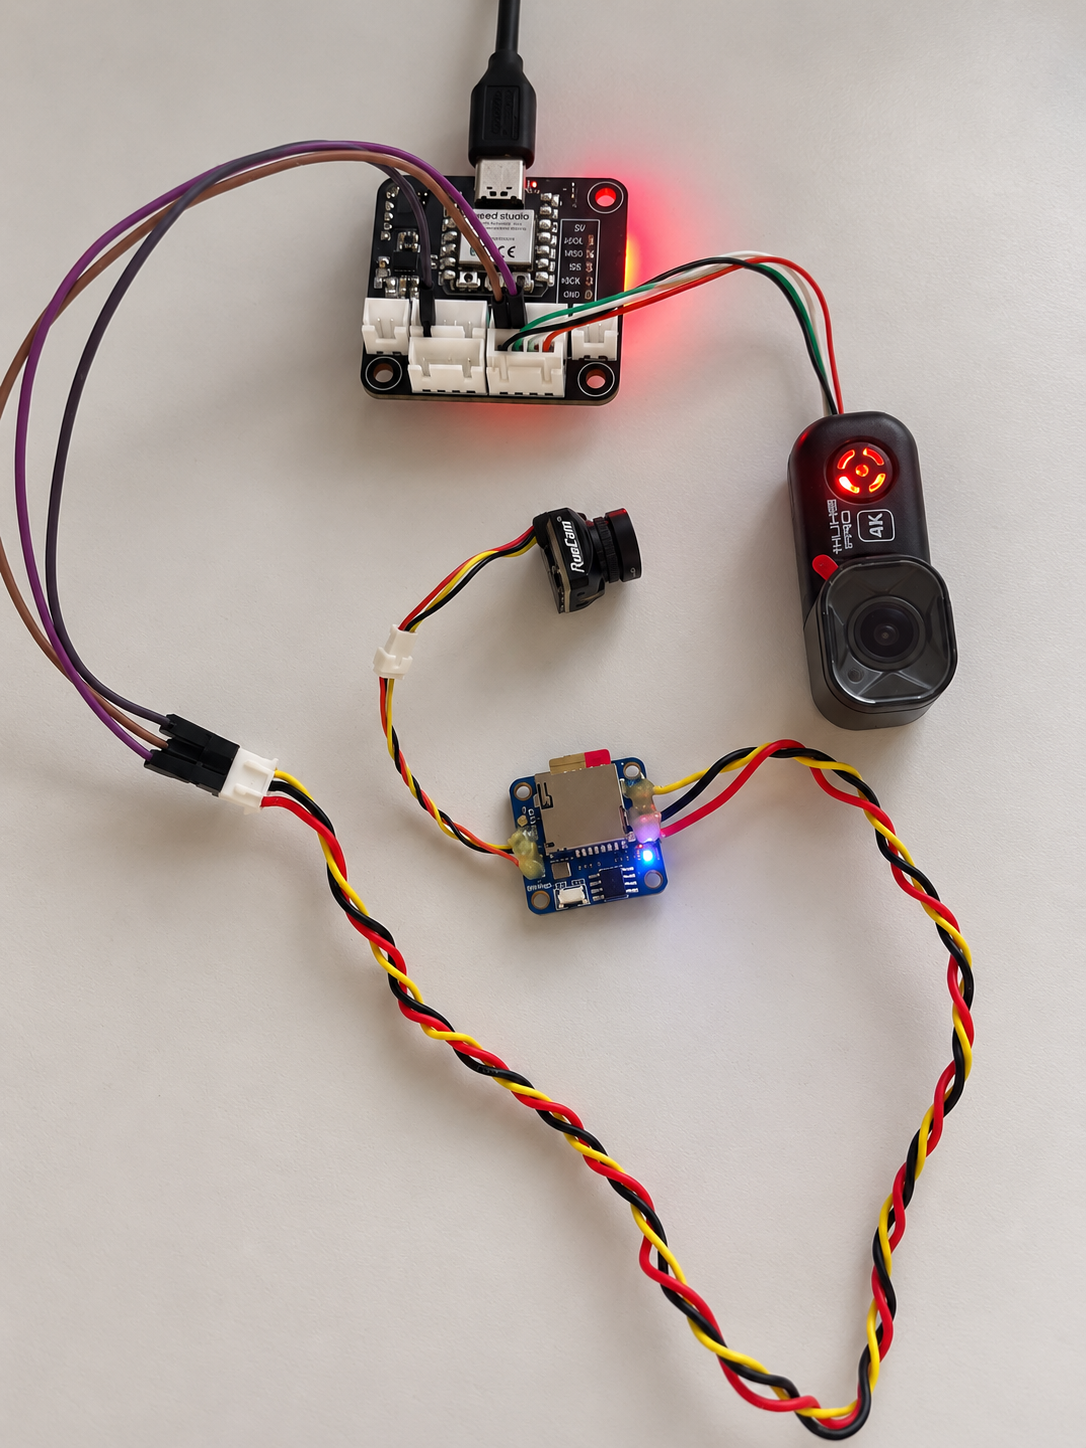
\includegraphics[width=0.82\textwidth]{figures/tests_cameras.PNG}
    \caption{Essais au sol du système de caméras.}
    \label{fig:tests_cameras}
\end{figure}

\newpage
